\documentclass[11pt,]{article}
\usepackage{lmodern}
\usepackage{amssymb,amsmath}
\usepackage{ifxetex,ifluatex}
\usepackage{fixltx2e} % provides \textsubscript
\ifnum 0\ifxetex 1\fi\ifluatex 1\fi=0 % if pdftex
  \usepackage[T1]{fontenc}
  \usepackage[utf8]{inputenc}
\else % if luatex or xelatex
  \ifxetex
    \usepackage{mathspec}
  \else
    \usepackage{fontspec}
  \fi
  \defaultfontfeatures{Ligatures=TeX,Scale=MatchLowercase}
\fi
% use upquote if available, for straight quotes in verbatim environments
\IfFileExists{upquote.sty}{\usepackage{upquote}}{}
% use microtype if available
\IfFileExists{microtype.sty}{%
\usepackage{microtype}
\UseMicrotypeSet[protrusion]{basicmath} % disable protrusion for tt fonts
}{}
\usepackage[margin=1.0in]{geometry}
\usepackage{hyperref}
\hypersetup{unicode=true,
            pdftitle={NAME OF THIS STUDY},
            pdfborder={0 0 0},
            breaklinks=true}
\urlstyle{same}  % don't use monospace font for urls
\usepackage{graphicx,grffile}
\makeatletter
\def\maxwidth{\ifdim\Gin@nat@width>\linewidth\linewidth\else\Gin@nat@width\fi}
\def\maxheight{\ifdim\Gin@nat@height>\textheight\textheight\else\Gin@nat@height\fi}
\makeatother
% Scale images if necessary, so that they will not overflow the page
% margins by default, and it is still possible to overwrite the defaults
% using explicit options in \includegraphics[width, height, ...]{}
\setkeys{Gin}{width=\maxwidth,height=\maxheight,keepaspectratio}
\IfFileExists{parskip.sty}{%
\usepackage{parskip}
}{% else
\setlength{\parindent}{0pt}
\setlength{\parskip}{6pt plus 2pt minus 1pt}
}
\setlength{\emergencystretch}{3em}  % prevent overfull lines
\providecommand{\tightlist}{%
  \setlength{\itemsep}{0pt}\setlength{\parskip}{0pt}}
\setcounter{secnumdepth}{0}
% Redefines (sub)paragraphs to behave more like sections
\ifx\paragraph\undefined\else
\let\oldparagraph\paragraph
\renewcommand{\paragraph}[1]{\oldparagraph{#1}\mbox{}}
\fi
\ifx\subparagraph\undefined\else
\let\oldsubparagraph\subparagraph
\renewcommand{\subparagraph}[1]{\oldsubparagraph{#1}\mbox{}}
\fi

%%% Use protect on footnotes to avoid problems with footnotes in titles
\let\rmarkdownfootnote\footnote%
\def\footnote{\protect\rmarkdownfootnote}

%%% Change title format to be more compact
\usepackage{titling}

% Create subtitle command for use in maketitle
\newcommand{\subtitle}[1]{
  \posttitle{
    \begin{center}\large#1\end{center}
    }
}

\setlength{\droptitle}{-2em}

  \title{\textbf{NAME OF THIS STUDY}}
    \pretitle{\vspace{\droptitle}\centering\huge}
  \posttitle{\par}
    \author{}
    \preauthor{}\postauthor{}
    \date{}
    \predate{}\postdate{}
  
\usepackage{booktabs}
\usepackage{longtable}
\usepackage{array}
\usepackage{multirow}
\usepackage[table]{xcolor}
\usepackage{wrapfig}
\usepackage{float}
\usepackage{colortbl}
\usepackage{pdflscape}
\usepackage{tabu}
\usepackage{threeparttable}
\usepackage{threeparttablex}
\usepackage[normalem]{ulem}
\usepackage{makecell}

\usepackage{helvet} % Helvetica font
\renewcommand*\familydefault{\sfdefault} % Use the sans serif version of the font
\usepackage[T1]{fontenc}

\usepackage[none]{hyphenat}

\usepackage{setspace}
\doublespacing
\setlength{\parskip}{1em}

\usepackage{lineno}

\usepackage{pdfpages}

\begin{document}
\maketitle

\vspace{35mm}

Running title: INSERT RUNNING TITLE HERE

\vspace{35mm}

Begüm D. Topçuoğlu\^{}1, Jenna Wiens\^{}2, Patrick D.
Schloss\textsuperscript{1\(\dagger\)}

\vspace{40mm}

\(\dagger\) To whom correspondence should be addressed:
\href{mailto:pschloss@umich.edu}{\nolinkurl{pschloss@umich.edu}}

1. Department of Microbiology and Immunology, University of Michigan,
Ann Arbor, MI 48109

2. Department of Computer Science and Engineering, University or
Michigan, Ann Arbor, MI 49109

\newpage

\linenumbers

\subsection{Abstract}\label{abstract}

\newpage

\subsection{Introduction}\label{introduction}

As gut microbiome field continues to grow, there will be an
ever-increasing demand for reproducible machine learning methods to
analyze microbiome sequence read count data and to determine association
with a continuous or categorical phenotype of interest.

Colorectal cancer is one of the leading cause of death among cancers in
the United States. Early diagnosis increases the chance of survival.
However the current diagnostic methods are expensive and invasive. As a
less invasive tool, numerous studies use relative abundances of the gut
bacteria populations to predict disease progression. Most microbial
communities are pretty patchy and the likelihood of a single feature
that explains the differences in health is pretty small. It is likely
that many biomarkers are needed to account for the patchiness as well as
the context dependency of the features.

ML use in microbiome literature is a bit like the wild west with lack of
clarity over methods, testing, validation, etc. There is a need for
guidance on how to properly implement these different methods. We need
to emphasize good machine learning practices and pipelines and discuss
the reproducibility, robustness and actionability of models.

We established a non-leaky pipeline. We performed L1 and L2-regularized
logistic regression, Linear SVM, Non-Linear SVM, Decision tree, Random
forest, XGBoost and Feed Forward Neural Net classification models. We
evaluated the classification performance of different machine learning
methods. We also want to discuss the reproducibility, robustness,
actionability, interpretibility and susceptibility to overfitting of
each method.

Generalisation Perfomance of each model. Is there a maximum threshold of
prediction with all these methods? Does an increase in model complexity
improve predictibility? Synthesis statement regarding modeling 16S
microbiome data

\subsection{Results and Discussion}\label{results-and-discussion}

\subsection{Conclusions}\label{conclusions}

\subsection{Materials and Methods}\label{materials-and-methods}

\newpage

\textbf{Figure 1. Generalization and classification performance of
modeling methods } AUC values of all cross validation and testing
performances.

\begin{center}
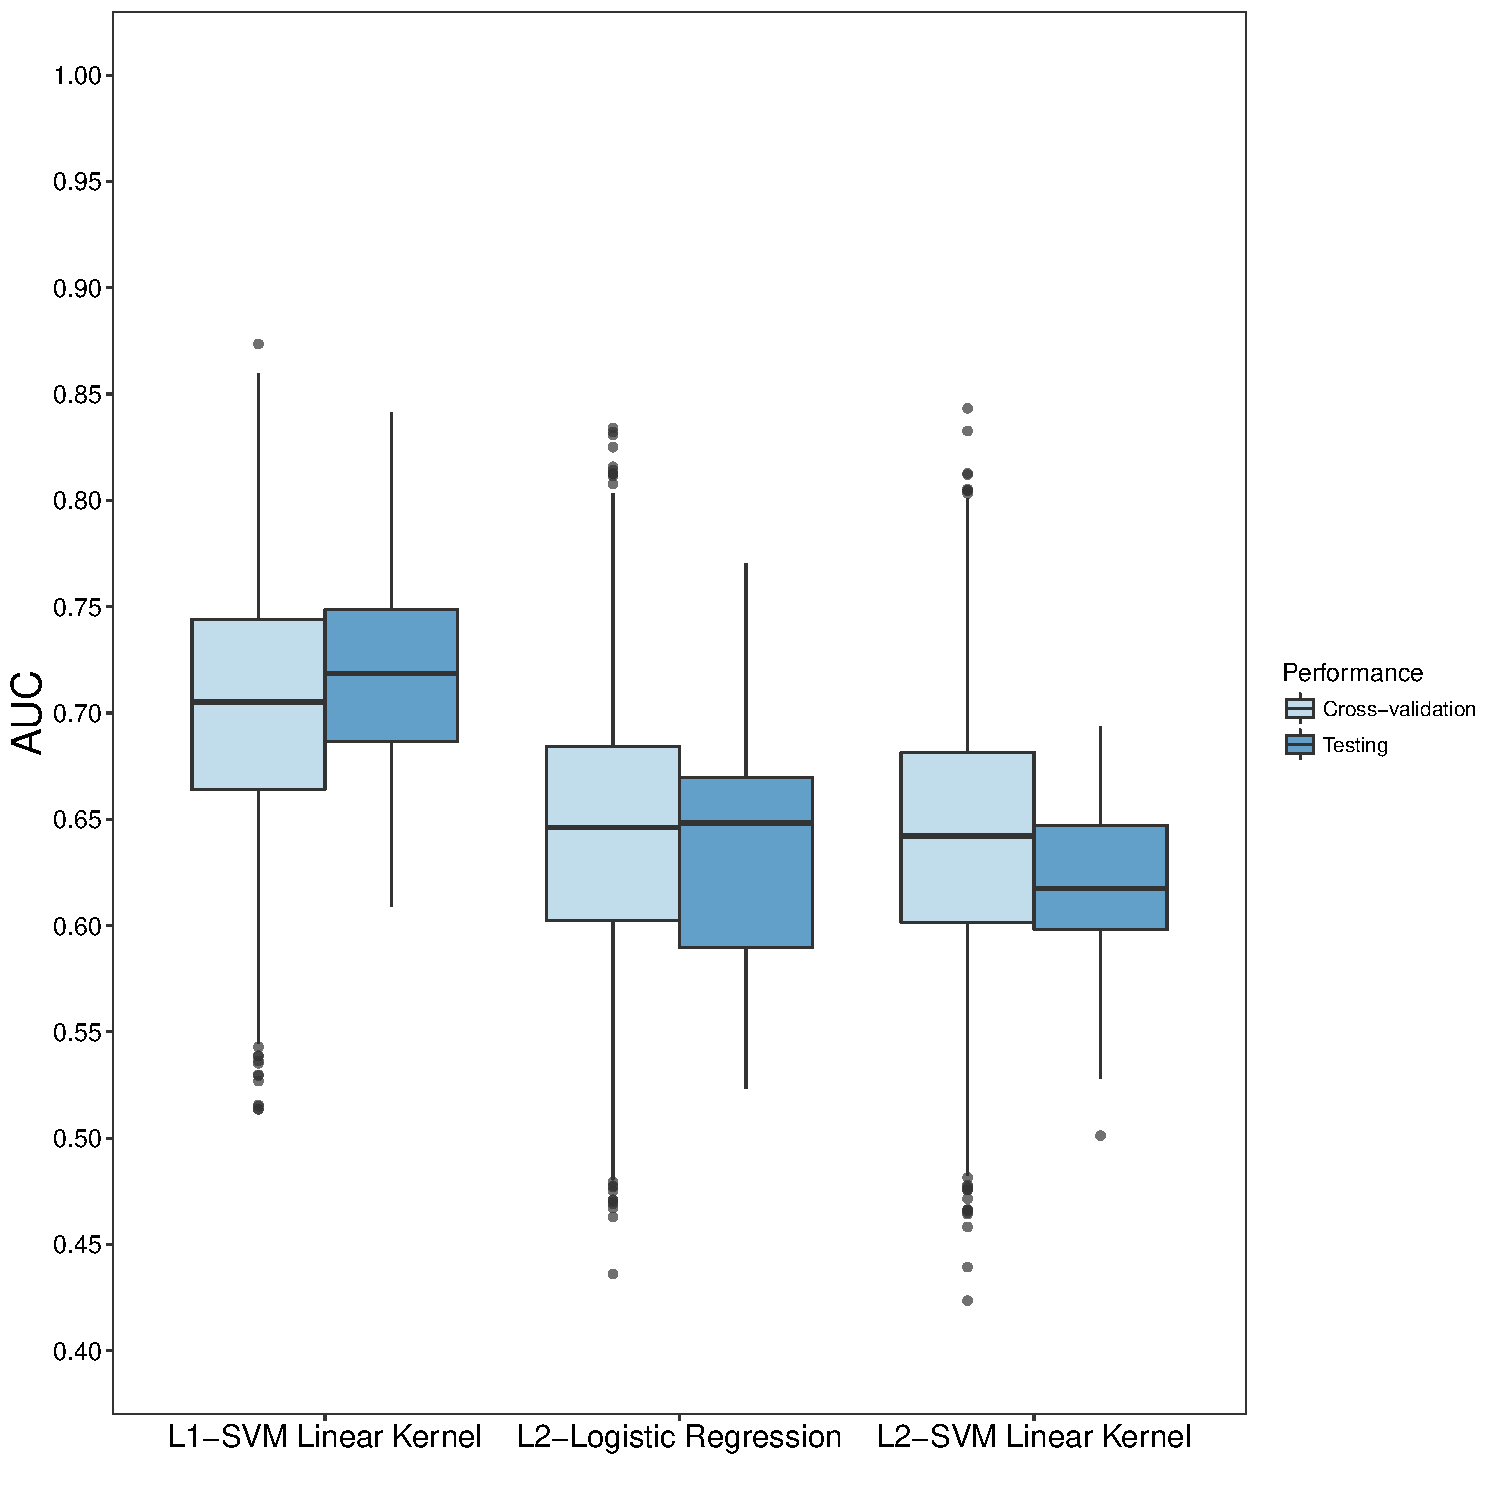
\includegraphics[width=7in]{../results/figures/AUC_comparison.pdf}
\end{center}

\rowcolors{2}{gray!6}{white}

\begin{table}

\caption{\label{tab:table_1_models}Optimized hyper-parameters, pre-processing and cross-validation methods and software implementation of the classification algorithms.}
\resizebox{\linewidth}{!}{
\begin{tabular}[t]{>{\raggedright\arraybackslash}p{10em}>{\raggedright\arraybackslash}p{8em}>{\raggedright\arraybackslash}p{9em}r>{\raggedright\arraybackslash}p{5em}l}
\hiderowcolors
\toprule
\textbf{Method} & \textbf{Parameter} & \textbf{Cross Validation} & \textbf{Epoch} & \textbf{Scaler} & \textbf{Sklearn Function}\\
\midrule
\showrowcolors
\multicolumn{1}{>{\raggedright\arraybackslash}p{10em}}{Logistic Regression} & \multicolumn{1}{>{\raggedright\arraybackslash}p{8em}}{C} & \multicolumn{1}{>{\raggedright\arraybackslash}p{9em}}{5-fold, 100-repeats} & \multicolumn{1}{l}{100} & \multicolumn{1}{>{\raggedright\arraybackslash}p{5em}}{MinMax} & \multicolumn{1}{l}{LogisticRegression}\\
\multicolumn{1}{>{\raggedright\arraybackslash}p{10em}}{L1 SVM Linear Kernel} & \multicolumn{1}{>{\raggedright\arraybackslash}p{8em}}{C} & \multicolumn{1}{>{\raggedright\arraybackslash}p{9em}}{5-fold, 100-repeats} & \multicolumn{1}{l}{100} & \multicolumn{1}{>{\raggedright\arraybackslash}p{5em}}{Standard} & \multicolumn{1}{l}{LinearSVC}\\
\multicolumn{1}{>{\raggedright\arraybackslash}p{10em}}{L2 SVM Linear Kernel} & \multicolumn{1}{>{\raggedright\arraybackslash}p{8em}}{C} & \multicolumn{1}{>{\raggedright\arraybackslash}p{9em}}{5-fold, 100-repeats} & \multicolumn{1}{l}{100} & \multicolumn{1}{>{\raggedright\arraybackslash}p{5em}}{Standard} & \multicolumn{1}{l}{LinearSVC}\\
\multicolumn{1}{>{\raggedright\arraybackslash}p{10em}}{SVM RBF Kernel} & \multicolumn{1}{>{\raggedright\arraybackslash}p{8em}}{C, gamma} & \multicolumn{1}{>{\raggedright\arraybackslash}p{9em}}{5-fold, 100-repeats} & \multicolumn{1}{l}{100} & \multicolumn{1}{>{\raggedright\arraybackslash}p{5em}}{Standard} & \multicolumn{1}{l}{SVC}\\
\multicolumn{1}{>{\raggedright\arraybackslash}p{10em}}{Decision Tree} & \multicolumn{1}{>{\raggedright\arraybackslash}p{8em}}{max\_depth, min\_samples\_split} & \multicolumn{1}{>{\raggedright\arraybackslash}p{9em}}{5-fold, 100-repeats} & \multicolumn{1}{l}{100} & \multicolumn{1}{>{\raggedright\arraybackslash}p{5em}}{MinMax} & \multicolumn{1}{l}{DecisionTreeClassifier}\\
\multicolumn{1}{>{\raggedright\arraybackslash}p{10em}}{Random Forest} & \multicolumn{1}{>{\raggedright\arraybackslash}p{8em}}{n\_estimators, max\_features} & \multicolumn{1}{>{\raggedright\arraybackslash}p{9em}}{5-fold, 100-repeats} & \multicolumn{1}{l}{100} & \multicolumn{1}{>{\raggedright\arraybackslash}p{5em}}{MinMax} & \multicolumn{1}{l}{RandomForestClassifier}\\
\multicolumn{1}{>{\raggedright\arraybackslash}p{10em}}{XGBoost} & \multicolumn{1}{>{\raggedright\arraybackslash}p{8em}}{n\_estimators, colsample\_bytree, learning\_rate, subsample, max\_depth, min\_child\_weight} & \multicolumn{1}{>{\raggedright\arraybackslash}p{9em}}{5-fold, 100-repeats} & \multicolumn{1}{l}{100} & \multicolumn{1}{>{\raggedright\arraybackslash}p{5em}}{MinMax} & \multicolumn{1}{l}{XGBClassifier}\\
\bottomrule
\end{tabular}}
\end{table}

\rowcolors{2}{white}{white}

\rowcolors{1}{white}{gray!6}

\begin{table}

\caption{\label{tab:table_2_3_params}The range of optimized hyper-parameters for logistic regression and support vector machines.}
\resizebox{\linewidth}{!}{
\begin{tabular}[t]{l|>{}llll|>{}llll|>{}lll|>{}lllll}
\hiderowcolors
\toprule
\multicolumn{1}{c}{\bfseries Parameter} & \multicolumn{4}{c}{\bfseries L2 Logistic} & \multicolumn{4}{c}{\bfseries L1 SVM Linear} & \multicolumn{3}{c}{\bfseries L2 SVM Linear } & \multicolumn{5}{c}{\bfseries SVM RBF} \\
\cmidrule(l{2pt}r{2pt}){1-1} \cmidrule(l{2pt}r{2pt}){2-5} \cmidrule(l{2pt}r{2pt}){6-9} \cmidrule(l{2pt}r{2pt}){10-12} \cmidrule(l{2pt}r{2pt}){13-17}
\showrowcolors
C & 0.01 & 0.1 & 1 & 10 & 0.001 & 0.01 & 0.1 & 1 & 0.01 & 0.1 & 1 & 1e-06 & 1e-05 & 1e-04 & 0.001 & 0.01\\
gamma & - & - & - & - & - & - & - & - & - & - & - & 1e-09 & 1e-08 & 1e-07 & - & -\\
\bottomrule
\end{tabular}}
\end{table}

\rowcolors{2}{white}{white}

\rowcolors{1}{white}{gray!6}

\begin{table}

\caption{\label{tab:table_2_3_params}The range of optimized hyper-parameters for tree based classification algorithms.}
\resizebox{\linewidth}{!}{
\fontsize{6}{8}\selectfont
\begin{tabular}[t]{l|>{}lllll|>{}llll|>{}lll}
\hiderowcolors
\toprule
\multicolumn{1}{c}{\bfseries Parameter} & \multicolumn{5}{c}{\bfseries Random Forest} & \multicolumn{4}{c}{\bfseries Decision Tree} & \multicolumn{3}{c}{\bfseries XGBoost} \\
\cmidrule(l{2pt}r{2pt}){1-1} \cmidrule(l{2pt}r{2pt}){2-6} \cmidrule(l{2pt}r{2pt}){7-10} \cmidrule(l{2pt}r{2pt}){11-13}
\showrowcolors
learning\_rate & - & - & - & - & - & - & - & - & - & 0.01 & 0.1 & 1\\
max\_depth & - & - & - & - & - & 6 & 8 & 10 & 50 & 6 & 7 & 8\\
max\_features & 10 & 80 & 500 & 1000 & 1500 & - & - & - & - & - & - & -\\
min\_child\_weight & - & - & - & - & - & - & - & - & - & 1 & 2 & 3\\
min\_samples\_split & - & - & - & - & - & 10 & 25 & 50 & - & - & - & -\\
n\_estimators & 1000 & - & - & - & - & - & - & - & - & 100 & - & -\\
subsample & - & - & - & - & - & - & - & - & - & 0.7 & 0.8 & 0.9\\
\bottomrule
\end{tabular}}
\end{table}

\rowcolors{2}{white}{white}


\end{document}
